\documentclass[10pt]{beamer}
\usetheme{metropolis}
\usecolortheme{default}
\usepackage{tcolorbox}
\usepackage{booktabs}
\usepackage{amsmath}
\usepackage{graphicx}
\usepackage{tikz}
\usepackage{pgfplots}
\pgfplotsset{compat=1.17}
\usetikzlibrary{arrows.meta, positioning, calc, shapes, fit, backgrounds}
\definecolor{myTeal}{HTML}{23373b}
\definecolor{myOrange}{HTML}{EB811B}
\setbeamercolor{alerted text}{fg=myOrange}


\title{Political Competition and Macroeconomic Performance}
\subtitle{ECO1028 – Politics Without Romance}
\author{Beatriz Gietner\\
\texttt{beatriz.gietner@dcu.ie}}
\date{\today}

\begin{document}

\maketitle

\begin{frame}{Outline}
\tableofcontents
\end{frame}



\section{Do Governments Manipulate Budgets for Votes?}

\begin{frame}{Before We Begin: A Diagnostic Question}
\textbf{Quick poll – imagine a government facing an election in 6 months:}

\begin{itemize}
\item What do you expect to happen to the \alert{budget balance}?
\begin{itemize}
\item A) Deficit \emph{increases}
\item B) Deficit \emph{decreases}
\item C) No systematic change
\end{itemize}
\end{itemize}

\vspace{0.5cm}
\alert{Follow-up:} If A, \emph{how} do you think this happens?
\begin{itemize}
\item More spending?
\item Lower taxes?
\item Targeted projects?
\end{itemize}

\vspace{0.5cm}
\textbf{Today's question:} Are these patterns systematic or just political folklore?
\end{frame}


\begin{frame}{The Central Puzzle}
\textbf{Two basic facts:}

\begin{itemize}
\item Voters care about economic outcomes
\item Politicians care about re-election
\end{itemize}

\vspace{0.5cm}
\alert{If voters reward "good" economic performance,}
politicians have incentives to \emph{shape} those outcomes.

\vspace{0.5cm}
\textbf{Public Choice perspective:}
\begin{itemize}
\item Politicians are not benevolent planners
\item They respond to incentives and constraints
\end{itemize}
\end{frame}


\begin{frame}{Why Budgets Are Politically Powerful}
\textbf{Budgets are the main policy instrument governments control:}

\begin{itemize}
\item Taxes
\item Transfers
\item Public investment
\item Public sector wages
\end{itemize}

\vspace{0.5cm}
\textbf{They are:}
\begin{itemize}
\item Highly visible
\item Easily targeted
\item Adjustable within one fiscal year
\end{itemize}

\vspace{0.5cm}
\alert{So if manipulation exists, budgets are the natural place to look.}
\end{frame}


\begin{frame}{From Economic Voting to Political Incentives}
\textbf{Well-known empirical regularity:}

\begin{itemize}
\item Incumbents perform better when the economy looks good
\end{itemize}

\vspace{0.5cm}
\textbf{Implication:}
\begin{itemize}
\item Governments have incentives to \alert{engineer} favourable conditions
\item Especially close to elections
\end{itemize}

\vspace{0.5cm}
\textbf{This is the logic behind:}
\begin{itemize}
\item Political business cycles
\item Political budget cycles
\end{itemize}
\end{frame}

\begin{frame}{Key Concepts: Political Budget Cycle}
\begin{tcolorbox}[colback=myTeal!5, colframe=myTeal, title=Definition]
\textbf{Political Budget Cycle (PBC):} Systematic manipulation of fiscal variables (spending, taxes, deficits) timed around elections to boost electoral support.
\end{tcolorbox}

\vspace{0.3cm}
\textbf{Related concept:}
\begin{itemize}
\item \textbf{Political Business Cycle:} Manipulation of macroeconomic outcomes (unemployment, growth) for electoral gain
\end{itemize}
\end{frame}

\begin{frame}{Public Choice Microfoundation: Competition for Pivotal Voters}
\textbf{A simple electoral logic:}

\begin{itemize}
\item Parties want office $\rightarrow$ they compete for votes.
\item With single-peaked preferences, both parties target the \alert{median (pivotal) voter}.
\item Economic policy becomes an input into vote choice.
\end{itemize}

\vspace{0.4cm}
\textbf{Implication for this lecture:}
\begin{itemize}
\item If fiscal/monetary policy shifts perceptions of competence or wellbeing,
incumbents have incentives to \alert{time} policy to maximise votes.
\end{itemize}

\vspace{0.2cm}
\textit{Downs (1957); standard Public Choice logic.}
\end{frame}


\begin{frame}{Opportunistic vs Partisan Incentives}
\textbf{Two competing views of political cycles:}

\begin{columns}
\begin{column}{0.48\textwidth}
\textbf{Opportunistic}
\begin{itemize}
\item All politicians want to win
\item Act the same before elections
\item Expand policy instruments
\end{itemize}
\end{column}

\begin{column}{0.48\textwidth}
\textbf{Partisan}
\begin{itemize}
\item Parties represent different voters
\item Left: low unemployment
\item Right: low inflation
\end{itemize}
\end{column}
\end{columns}

\vspace{0.4cm}
\alert{Mueller (Chapter 19): both mechanisms may coexist.}
\end{frame}

\begin{frame}{Opportunistic vs Partisan: Visual Summary}
\centering
\includegraphics[width=0.95\textwidth]{lecture3_models.JPG}

\vspace{0.3cm}
\footnotesize
\alert{Today's focus:} Opportunistic cycles, constrained by institutions.
\end{frame}



\begin{frame}{What We Will Learn}
\textbf{By the end of this lecture, you should understand:}

\begin{itemize}
\item Why early economists expected political cycles
\item Why output cycles are hard to detect
\item Why \alert{budget cycles} are more robust
\item How \alert{institutions} constrain manipulation
\end{itemize}

\vspace{0.5cm}
\textbf{Core readings:}
\begin{itemize}
\item \href{https://www.sciencedirect.com/science/article/pii/S004727270500143X}{Shi \& Svensson (2006): Political budget cycles: Do they differ across countries and why?}
\item \href{https://www.jstor.org/stable/2077833?seq=1}{Alesina \& Summers (1993): Central Bank Independence and Macroeconomic Performance: Some Comparative Evidence}
\end{itemize}
\end{frame}

\section{Why Did Economists Expect Political Cycles?}

\begin{frame}{The Original Political Business Cycle Story}
\textbf{Early intuition:}

\begin{itemize}
\item Voters like low unemployment and high growth
\item Politicians like re-election
\end{itemize}

\vspace{0.4cm}
\alert{So politicians try to "stimulate" the economy before elections,}
and accept the costs later.

\vspace{0.4cm}
\textbf{Prediction:}
\begin{itemize}
\item Pre-election expansion
\item Post-election contraction
\end{itemize}
\end{frame}


\begin{frame}{The Political Budget Cycle Pattern}
\centering
\includegraphics[width=0.9\textwidth]{lecture3_spendingcycle.JPG}

\vspace{0.3cm}
\footnotesize
\textbf{Key insight:} Budget deficits systematically increase before elections.
\end{frame}

\begin{frame}{The Short-Run Logic (Phillips Curve Intuition)}
\begin{tcolorbox}[colback=myTeal!5, colframe=myTeal, title=Definition]
\textbf{Phillips Curve:} Short-run trade-off between unemployment and inflation. Lower unemployment → higher inflation (and vice versa).
\end{tcolorbox}

\vspace{0.3cm}
\textbf{Political application:}
\begin{itemize}
\item Governments can temporarily reduce unemployment by accepting higher inflation
\item Costs (inflation) come later; benefits (jobs, growth) appear first
\end{itemize}

\vspace{0.3cm}
\alert{This creates an incentive to stimulate before elections.}
\end{frame}

\begin{frame}{Phillips Curve Trade-Off: The Temptation}
\centering
\includegraphics[width=0.85\textwidth]{lecture3_PC.JPG}

\vspace{0.3cm}
\footnotesize
Politicians can temporarily move from A to B - but only if voters don't anticipate it.
\end{frame}

\begin{frame}{Myopic Voters: The Simplest Case}
\textbf{Suppose voters are short-sighted:}

\begin{itemize}
\item They focus on current unemployment and growth
\item They heavily discount future inflation
\end{itemize}

\vspace{0.4cm}
\textbf{Then:}
\begin{itemize}
\item Incumbents can boost the economy before elections
\item Voters reward them at the polls
\end{itemize}

\vspace{0.4cm}
\alert{This is the original political business cycle.}
\end{frame}



\begin{frame}{But Something Goes Wrong}
\textbf{Two problems:}

\begin{itemize}
\item People are not completely naive
\item Expectations adjust
\end{itemize}

\vspace{0.4cm}
\textbf{If voters anticipate manipulation:}
\begin{itemize}
\item They demand higher wages
\item They revise expectations
\end{itemize}

\vspace{0.4cm}
\alert{Short-run gains disappear.}
\end{frame}


\begin{frame}{Why Rational Expectations Defeat Manipulation}
\centering
\includegraphics[width=0.9\textwidth]{lecture3_voters.png}

\vspace{0.3cm}
\footnotesize
\alert{Key result:} If voters anticipate the trade-off, output cycles disappear.
\end{frame}


\begin{frame}{The Missing Link: Competence Signaling}
\textbf{If voters are rational, why does manipulation work?}

\begin{itemize}
\item \textbf{Asymmetric information:} Voters cannot observe competence.
\item \textbf{The signal:} High spending and growth \emph{look} like ability.
\item \textbf{The trick:} Taxes and inflation come \emph{after} the election.
\end{itemize}

\vspace{0.3cm}
\textbf{Result:}
\begin{itemize}
\item Incumbents try to \alert{signal competence} by expanding spending
\item This creates future costs (debt, inflation, adjustment)
\item Which voters may not fully internalise
\end{itemize}

\vspace{0.2cm}
\alert{So manipulation can survive under imperfect information.}

\textit{\href{https://www.nber.org/system/files/working_papers/w2428/w2428.pdf}{Rogoff (1990)}; \href{https://www.sciencedirect.com/science/article/pii/S004727270500143X}{Shi \& Svensson (2006)};
\href{https://www.cato.org/sites/cato.org/files/pubs/pdf/pa594.pdf}{Caplan (2007)}}

\textit{Interpretation: electoral accountability with imperfect monitoring (principal-agent).}
\end{frame}

\begin{frame}{The Underlying Problem: Voters Can't Fully Monitor Politicians}
\textbf{Public Choice framing: a principal--agent problem}

\begin{itemize}
\item \textbf{Principals:} voters want good policy.
\item \textbf{Agents:} politicians want re-election (and sometimes rents).
\item \textbf{Friction:} voters observe outcomes imperfectly and with a lag.
\end{itemize}

\vspace{0.4cm}
\textbf{So manipulation can work when:}
\begin{itemize}
\item policy is \alert{visible now} (spending, tax cuts),
\item costs are \alert{less visible} or delayed (debt, inflation),
\item information is limited (media/institutions are weak).
\end{itemize}
\end{frame}


\begin{frame}{From Output Cycles to Budget Cycles}
\textbf{The empirical problem:}
\begin{itemize}
\item Output and unemployment cycles around elections are weak (especially in advanced democracies)
\end{itemize}

\vspace{0.3cm}
\alert{So where is the manipulation?}

\vspace{0.3cm}
\textbf{Modern shift:}
\begin{itemize}
\item Not "booms" and "busts"
\item But \alert{deficits, spending, and targeted transfers}
\end{itemize}

\vspace{0.3cm}
\textbf{Why budgets?} Politicians directly control them-they're visible and targetable.
\end{frame}

\section{Political Budget Cycles: Evidence}


\begin{frame}{What Is a Political Budget Cycle?}
\textbf{Definition:}
\begin{itemize}
\item A systematic increase in budget deficits around elections
\item Followed by post-election fiscal tightening
\end{itemize}

\vspace{0.3cm}
\textbf{Why focus on budgets?}

\begin{columns}
\begin{column}{0.48\textwidth}
Governments control:
\begin{itemize}
\item Public spending
\item Taxes
\item Transfers
\end{itemize}
\end{column}

\begin{column}{0.48\textwidth}
They don't control:
\begin{itemize}
\item Growth
\item Employment
\item External shocks
\end{itemize}
\end{column}
\end{columns}

\vspace{0.3cm}
\alert{So if manipulation exists, it should appear in budgets.}
\end{frame}

\begin{frame}{Shi \& Svensson (2006): Research Design}
\textbf{The question:} Do political budget cycles exist?

\vspace{0.2cm}
\textbf{If yes:}
\begin{itemize}
\item Are they larger in some countries?
\item What explains the differences?
\end{itemize}

\vspace{0.3cm}
\textbf{Dataset:}
\begin{itemize}
\item Large panel of countries (democratic and non-democratic)
\item Multiple election cycles
\item Key outcome: Fiscal deficit as \% of GDP
\end{itemize}
\end{frame}


\begin{frame}{Identification Strategy}
\textbf{The problem:}
\begin{itemize}
\item Governments may call elections when the economy is already good
\item We must separate manipulation from strategic election timing
\end{itemize}

\vspace{0.3cm}
\textbf{The solution:}
\begin{itemize}
\item Distinguish between:
\begin{itemize}
\item \textbf{Predetermined} elections (fixed dates)
\item \textbf{Endogenous} elections (PM chooses timing)
\end{itemize}
\end{itemize}

\vspace{0.3cm}
\alert{Logic:} If cycles appear even with predetermined elections, they're less likely driven by timing alone.
\end{frame}


\begin{frame}{Competence Signaling: The Mechanism}
\centering
\includegraphics[width=0.85\textwidth]{lecture3_polschoice.JPG}

\vspace{0.3cm}
\footnotesize
\textbf{Modern insight:} Politicians use \alert{spending} as a signal of competence when voters have imperfect information (Rogoff 1990; \href{https://www.sciencedirect.com/science/article/pii/S004727270500143X}{Shi \& Svensson 2006}).
\end{frame}

\begin{frame}{Identification: Predetermined vs Endogenous Elections}
\centering
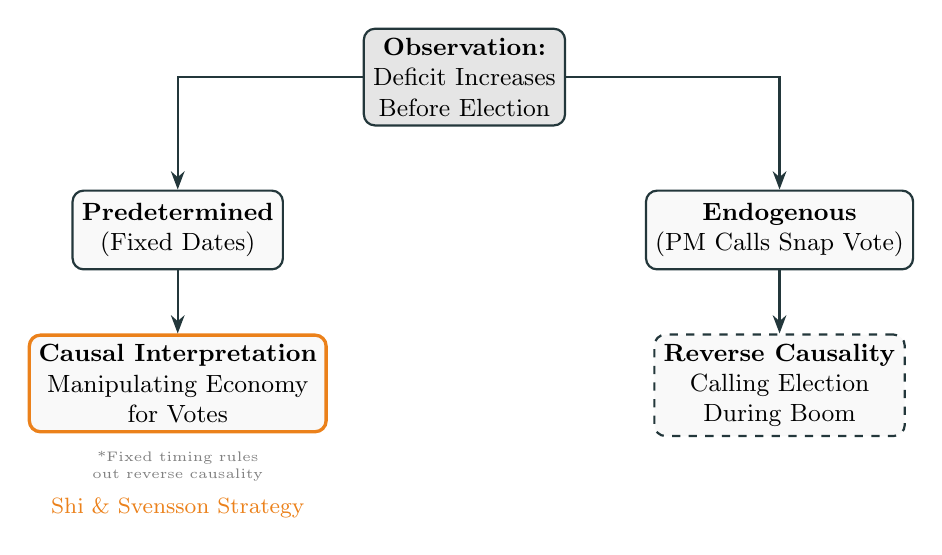
\begin{tikzpicture}[
node distance=0.8cm and 0.5cm,
box/.style={rectangle, draw=myTeal, fill=gray!5, rounded corners, thick, align=center, minimum width=2.5cm, minimum height=1cm, font=\small},
arrow/.style={-{Stealth}, thick, myTeal}
]

\node[box, fill=gray!20] (start) {\textbf{Observation:}\\Deficit Increases\\Before Election};

\node[box, below left=of start, xshift=-0.5cm] (predet) {\textbf{Predetermined}\\(Fixed Dates)};
\node[box, below right=of start, xshift=0.5cm] (endog) {\textbf{Endogenous}\\(PM Calls Snap Vote)};

\node[box, below=of predet, draw=myOrange, very thick] (concl1) {\textbf{Causal Interpretation}\\Manipulating Economy\\for Votes};
\node[box, below=of endog, dashed] (concl2) {\textbf{Reverse Causality}\\Calling Election\\During Boom};

\node[below=0.1cm of concl1, text=gray, font=\tiny, align=center, text width=3cm] {*Fixed timing rules out reverse causality};

\draw[arrow] (start) -| (predet);
\draw[arrow] (start) -| (endog);
\draw[arrow] (predet) -- (concl1);
\draw[arrow] (endog) -- (concl2);

\node[below=0.3cm of concl1, text=myOrange, font=\footnotesize, yshift=-0.4cm] {Shi \& Svensson Strategy};
\end{tikzpicture}
\end{frame}


\begin{frame}{Main Findings}
\textbf{Headline result:}
\begin{itemize}
\item Government deficits rise in election years
\item By almost \alert{1\% of GDP} on average
\end{itemize}

\vspace{0.4cm}
\textbf{Key heterogeneity:}
\begin{itemize}
\item Political budget cycles are \alert{much larger} in developing countries
\end{itemize}

\vspace{0.3cm}
\alert{Question:} Why the difference?
\end{frame}


\begin{frame}{The Institutional Explanation}
\textbf{Two core mechanisms:}

\begin{enumerate}
\item \textbf{Political rents}
\item \textbf{Share of informed voters}
\end{enumerate}

\vspace{0.4cm}
\alert{Institutions determine how easy manipulation is.}
\end{frame}

\begin{frame}{Measuring the Mechanism}
\textbf{How do Shi \& Svensson measure institutions?}

\begin{itemize}
\item \textbf{Information:}
\begin{itemize}
\item Radios per capita
\item Freedom of broadcasting
\end{itemize}

\item \textbf{Rents:}
\begin{itemize}
\item Corruption indices
\item Protection against expropriation
\end{itemize}
\end{itemize}

\vspace{0.4cm}
\textbf{Finding:}
\begin{itemize}
\item High info + Low rents $\rightarrow$ No cycle
\item Low info + High rents $\rightarrow$ Large cycle
\end{itemize}
\end{frame}

\begin{frame}{Two Mechanisms Behind Heterogeneity}
\textbf{1. Political Rents}
\begin{itemize}
\item Private benefits politicians get from staying in office
\item If rents are high → politicians distort policy more
\end{itemize}

\vspace{0.3cm}
\textbf{2. Voter Information}
\begin{itemize}
\item If many voters are informed → they see through manipulation
\item If many voters are uninformed → manipulation succeeds
\end{itemize}

\vspace{0.3cm}
\alert{Result:} High rents + Low information = Large cycles
\end{frame}

\begin{frame}{Public Choice Interpretation}
\textbf{What this means:}
\begin{itemize}
\item Political competition alone does not prevent manipulation
\item \alert{Institutions} determine the size of the problem
\end{itemize}

\vspace{0.4cm}
\textbf{Core message:}
\begin{itemize}
\item Politicians respond to incentives
\item Voters respond to information
\item Institutions shape both
\end{itemize}
\end{frame}

\begin{frame}{Institutional Quality and Budget Cycle Size}
\centering
\includegraphics[width=0.9\textwidth]{lecture3_budgetcycle.JPG}

\vspace{0.3cm}
\footnotesize
\textbf{Empirical finding:} Budget cycles are larger in countries with weaker institutions (\href{https://www.sciencedirect.com/science/article/pii/S004727270500143X}{Shi \& Svensson 2006}; \href{https://www.sciencedirect.com/science/article/pii/S0304393205000887}{Brender \& Drazen 2005}).
\end{frame}

\section{Time Inconsistency and Inflation Bias}

\begin{frame}{Key Concepts: Time Inconsistency}
\begin{tcolorbox}[colback=myTeal!5, colframe=myTeal, title=Definition]
\textbf{Time Inconsistency:} A situation where a policy that is optimal to announce ex-ante becomes suboptimal to implement ex-post.
\end{tcolorbox}

\vspace{0.3cm}
\textbf{In monetary policy:}
\begin{itemize}
\item \textit{Ex ante:} Central bank promises low inflation
\item \textit{Ex post:} Central bank has incentive to inflate (reduce unemployment)
\item Result: Nobody believes the promise $\rightarrow$ high inflation, no gain
\end{itemize}
\end{frame}

\begin{frame}{The Time Inconsistency Problem}
\textbf{Politicians may also try to influence monetary policy:}

\vspace{0.3cm}
\textbf{The temptation:}
\begin{itemize}
\item Government promises low inflation
\item After wages and contracts are set, it has an incentive to create surprise inflation
\end{itemize}

\vspace{0.4cm}
\alert{But rational agents anticipate this.}
\end{frame}


\begin{frame}{Inflation Bias and the Commitment Problem}
\textbf{If people expect manipulation:}
\begin{itemize}
\item They demand higher wages
\item Firms raise prices
\end{itemize}

\vspace{0.3cm}
\textbf{Result:}
\begin{itemize}
\item No long-run gain in output or employment
\item Permanently higher inflation
\end{itemize}

\vspace{0.3cm}
\alert{This is the inflation bias.}

\vspace{0.3cm}
\textbf{Why promises don't work:}
\begin{itemize}
\item Governments cannot credibly commit
\item Future incentives differ from current promises
\end{itemize}
\end{frame}

\begin{frame}{Institutional Solution: Central Bank Independence}
\textbf{If politicians cannot commit, they can delegate to an independent authority.}

\vspace{0.3cm}
\textbf{An independent central bank:}
\begin{itemize}
\item Sets monetary policy without political pressure
\item Has long, protected terms for governors
\item Is legally insulated from the government
\end{itemize}

\vspace{0.3cm}
\alert{This motivates central bank independence (CBI).}
\end{frame}

\begin{frame}{Why Central Bank Independence?}
\begin{tcolorbox}[colback=myTeal!5, colframe=myTeal, title=Definition]
\textbf{Central Bank Independence (CBI):} Legal and operational autonomy of monetary authorities from political control, particularly over interest rate decisions.
\end{tcolorbox}

\vspace{0.3cm}
\textbf{The logic:}
\begin{itemize}
\item Politicians face re-election pressures
\item They prefer short-term growth over price stability
\item Independent central bank can commit credibly to low inflation
\end{itemize}

\vspace{0.3cm}
\alert{CBI solves the time inconsistency problem.}
\end{frame}

\begin{frame}{What Makes a Central Bank Independent?}
\textbf{CBI is measured by legal rules:}

\begin{enumerate}
\item \textbf{Appointments:}
\begin{itemize}
\item Who appoints the governor?
\item Are terms longer than electoral cycles?
\end{itemize}

\item \textbf{Budgetary freedom:}
\begin{itemize}
\item Can the government force the CB to buy its debt?
\end{itemize}

\item \textbf{Mission:}
\begin{itemize}
\item Is price stability the primary legal objective?
\end{itemize}
\end{enumerate}

\textit{\href{https://academic.oup.com/economicpolicy/article-abstract/6/13/341/2392405}{Grilli, Masciandaro \& Tabellini (1991)}; \href{https://www.jstor.org/stable/2077833?seq=1}{Alesina \& Summers (1993)}}
\end{frame}


\begin{frame}{Delegation as a Commitment Device}
\centering
\begin{columns}

\begin{column}{0.48\textwidth}
\centering
\textbf{Politician (Discretion)}
\vspace{0.3cm}

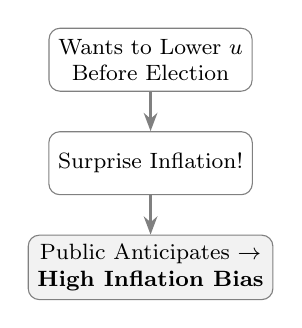
\begin{tikzpicture}[
box/.style={rectangle, draw=gray, rounded corners, align=center, font=\footnotesize, minimum width=2.5cm, minimum height=0.8cm},
arrow/.style={-{Stealth}, thick, gray}
]
\node[box] (obj) {Wants to Lower $u$\\Before Election};
\node[box, below=0.5cm of obj] (act) {Surprise Inflation!};
\node[box, below=0.5cm of act, fill=gray!10] (res) {Public Anticipates $\rightarrow$\\ \textbf{High Inflation Bias}};

\draw[arrow] (obj) -- (act);
\draw[arrow] (act) -- (res);
\end{tikzpicture}
\end{column}

\begin{column}{0.04\textwidth}
\end{column}

\begin{column}{0.48\textwidth}
\centering
\textbf{Independent CB (Rule)}
\vspace{0.3cm}

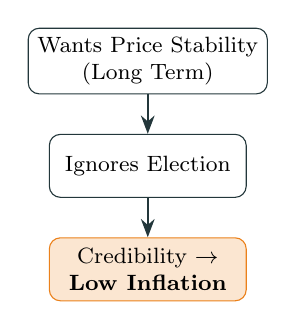
\begin{tikzpicture}[
box/.style={rectangle, draw=myTeal, rounded corners, align=center, font=\footnotesize, minimum width=2.5cm, minimum height=0.8cm},
arrow/.style={-{Stealth}, thick, myTeal}
]
\node[box] (obj) {Wants Price Stability\\(Long Term)};
\node[box, below=0.5cm of obj] (act) {Ignores Election};
\node[box, below=0.5cm of act, fill=myOrange!20, draw=myOrange] (res) {Credibility $\rightarrow$\\ \textbf{Low Inflation}};

\draw[arrow] (obj) -- (act);
\draw[arrow] (act) -- (res);
\end{tikzpicture}
\end{column}
\end{columns}

\vspace{0.5cm}
\footnotesize
\alert{Key lesson:} Delegation to independent institutions solves time-inconsistency (\href{https://academic.oup.com/qje/article-abstract/100/4/1169/1895960}{Rogoff 1985}; \href{https://www.jstor.org/stable/2077833?seq=1}{Alesina \& Summers 1993}).
\end{frame}


\begin{frame}{Alesina \& Summers (1993): Research Design}
\textbf{The question:}
\begin{itemize}
\item Do independent central banks reduce inflation?
\item Without harming growth or employment?
\end{itemize}

\vspace{0.3cm}
\textbf{Approach:}
\begin{itemize}
\item Cross-country comparison
\item Measures of legal central bank independence
\item Inflation, growth, unemployment outcomes
\end{itemize}
\end{frame}


\begin{frame}{Main Findings: CBI Works}
\textbf{Inflation:}
\begin{itemize}
\item Countries with more independent central banks
\item Have \alert{significantly lower inflation}
\end{itemize}

\vspace{0.4cm}
\textbf{Real outcomes:}
\begin{itemize}
\item No systematic evidence of:
\begin{itemize}
\item Lower growth
\item Higher unemployment
\end{itemize}
\end{itemize}

\vspace{0.3cm}
\alert{Price stability appears to come without a real cost.}
\end{frame}


\begin{frame}{Why CBI Works: Parallel with Budget Cycles}
\textbf{CBI works because:}
\begin{itemize}
\item It removes short-run political incentives
\item It creates credibility
\item Expectations adjust accordingly
\end{itemize}

\vspace{0.4cm}
\textbf{Common structure:}
\begin{itemize}
\item Politicians face short-run temptations
\item Society faces long-run costs
\item Institutions reduce the scope for manipulation
\end{itemize}
\end{frame}

\section{Fiscal Policy Cycles and Composition}

\begin{frame}{Beyond Deficits: How Is Fiscal Policy Manipulated?}
\textbf{So far:} election years → higher deficits.

\vspace{0.4cm}
\textbf{But deficits are aggregates.}

\vspace{0.4cm}
\alert{Which components of spending and taxation actually move?}
\end{frame}

\begin{frame}{Key Concept: Fiscal Policy Cycles}
\begin{tcolorbox}[colback=myTeal!5, colframe=myTeal, title=Definition]
\textbf{Fiscal Policy Cycles:} Systematic changes in the composition and timing of government spending and taxation around elections.
\end{tcolorbox}

\vspace{0.3cm}
\textbf{Relationship to other concepts:}
\begin{itemize}
\item \textbf{Political Business Cycles:} Focus on macro outcomes (GDP, unemployment)
\item \textbf{Political Budget Cycles:} Focus on deficits
\item \textbf{Fiscal Policy Cycles:} Focus on spending/tax composition
\end{itemize}

\vspace{0.3cm}
\alert{All three reflect the same incentive: manipulating policy for votes.}
\end{frame}

\begin{frame}{Nordhaus (1975): The Foundational Model}
\textbf{William Nordhaus (1975) proposed the first formal model of political business cycles.}

\vspace{0.3cm}
His key insight: Politicians exploit the Phillips curve trade-off between unemployment and inflation. Before elections, they stimulate the economy through expansionary monetary or fiscal policy, creating jobs and growth that boost their popularity. After winning re-election, they accept the inevitable costs - higher inflation - and contract the economy again.
   
The original model assumed voters have \alert{adaptive expectations} - they don't fully anticipate the manipulation. However, later work by Rogoff (1990) showed that cycles can persist even with rational voters, if there's asymmetric information about government competence.

\alert{Nordhaus gave us the "opportunistic politician" model that Schuknecht tests empirically in developing countries.}
\end{frame}

\begin{frame}{Schuknecht (2000): Why Focus on Spending Composition?}
\textbf{Why developing countries?}
\begin{itemize}
\item Weaker institutions
\item Smaller tax base
\item Greater scope for political discretion
\end{itemize}

\vspace{0.3cm}
\textbf{What can politicians easily manipulate?}

\begin{columns}
\begin{column}{0.48\textwidth}
\textbf{Taxes:}
\begin{itemize}
\item Slow to change
\item Administratively complex
\end{itemize}
\end{column}

\begin{column}{0.48\textwidth}
\textbf{Spending:}
\begin{itemize}
\item Faster to adjust
\item More visible
\item Easier to target
\end{itemize}
\end{column}
\end{columns}

\vspace{0.3cm}
\alert{So spending is the main vehicle for cycles.}
\end{frame}

\begin{frame}{Schuknecht (2000): What He Tests}
\textbf{Main hypotheses:}

\begin{itemize}
\item Expenditure rises in election years
\item Especially public investment
\item Taxes respond less
\end{itemize}
\end{frame}

\begin{frame}{Schuknecht (2000): Empirical Results}
\textbf{Sample:} 24 developing countries, 1973–1992

\vspace{0.3cm}
\textbf{Key findings:}
\begin{itemize}
\item Fiscal deficit increases by \alert{0.7\% of GDP} in election years
\item \alert{Two-thirds} of this is from spending increases
\item Only one-third from lower revenue
\end{itemize}

\vspace{0.3cm}
\textbf{Statistical significance:}
\begin{itemize}
\item \alert{Capital expenditure:} Significant at 5\% level
\item Current expenditure: Marginally significant (10\%)
\item Revenue: Not statistically significant
\end{itemize}

\vspace{0.3cm}
\alert{Bottom line:} Public investment is the main electoral tool.
\end{frame}

\begin{frame}{Why Politicians Prefer Public Investment}
\textbf{What makes capital spending politically attractive?}
\begin{itemize}
\item \textbf{Visibility:} Infrastructure projects are highly visible
\item \textbf{Targetability:} Can direct to swing districts
\item \textbf{Reversibility:} Easy to stop after election
\end{itemize}

\vspace{0.3cm}
\textbf{The political calculus:}
\begin{itemize}
\item Short-run electoral gains (jobs, contracts)
\item Long-run fiscal costs (maintenance, debt)
\item But those costs come after the election
\end{itemize}

\vspace{0.3cm}
\alert{Time-inconsistency in fiscal policy, not just monetary!}
\end{frame}

\begin{frame}{Schuknecht (2000): Institutional Constraints}
\textbf{What limits political budget cycles?}

\begin{itemize}
\item IMF-supported programs reduce expenditure growth
\item Trade-oriented economies face more constraints
\item Countries with fixed exchange rates have different patterns
\end{itemize}

\vspace{0.3cm}
\textbf{Policy implication:}
\begin{itemize}
\item Weak fiscal institutions facilitate cycles
\item Strengthening budget rules can reduce volatility
\item Similar to CBI for monetary policy
\end{itemize}

\vspace{0.3cm}
\alert{Institutions matter for constraining opportunistic behavior.}
\end{frame}

\begin{frame}{Composition of Spending: Visual Summary}
\centering
\includegraphics[width=0.85\textwidth]{lecture3_spendingcomp.JPG}

\vspace{0.3cm}
\footnotesize
\textbf{Composition matters:} Cycles show up more in \alert{visible, reversible} capital spending than in sticky current expenditures (Rogoff 1990).
\end{frame}


\section{Institutions, Incentives, and Performance}


\begin{frame}{Commitment Problems and Institutional Solutions}
\textbf{Two parallel problems:}

\begin{columns}
\begin{column}{0.48\textwidth}
\textbf{Fiscal policy}
\begin{itemize}
\item Election-year deficits
\item Spending manipulation
\end{itemize}
\end{column}

\begin{column}{0.48\textwidth}
\textbf{Monetary policy}
\begin{itemize}
\item Inflation bias
\item Surprise inflation
\end{itemize}
\end{column}
\end{columns}

\vspace{0.3cm}
\alert{Same structure: short-run gains vs long-run costs.}

\vspace{0.3cm}
\textbf{Institutional solutions:}
\begin{itemize}
\item Central bank independence
\item Fiscal rules, budget transparency
\item Independent fiscal councils
\end{itemize}
\end{frame}

\begin{frame}{Evolution of the Political Cycles Literature}
\textbf{When are cycles largest?}
\begin{itemize}
\item Weak institutions
\item High political rents
\item Low voter information
\end{itemize}

\vspace{0.3cm}
\textbf{Old vs Modern View:}

\begin{tabular}{p{0.45\textwidth} p{0.45\textwidth}}
\toprule
\textbf{Old PBC} & \textbf{Modern PBC} \\
\midrule
Output cycles & Budget cycles \\
Myopic voters & Information frictions \\
Inflation surprises & Deficits and spending \\
Macro trade-offs & Institutional constraints \\
\bottomrule
\end{tabular}
\end{frame}


\begin{frame}{Key Takeaways}
\begin{itemize}
\item Politicians face strong electoral incentives
\item Manipulation shows up in budgets, not output
\item Institutions constrain the size of cycles
\item Credibility solves commitment problems
\end{itemize}
\end{frame}


\begin{frame}{Discussion Questions}
\begin{itemize}
\item Would you trust politicians to self-restrain?
\item Are fiscal rules democratic or technocratic?
\item Should monetary policy be insulated from voters?
\end{itemize}
\end{frame}


\begin{frame}{Next Steps}
\textbf{Before next class:}
\begin{itemize}
\item Read the required papers
\item Think about Irish budget cycles
\end{itemize}

\end{frame}


\begin{frame}{Questions?}
\begin{center}
\Large Open discussion!
\end{center}
\end{frame}



\section{Irish Context: Budgets and Elections}

\begin{frame}{Do Political Budget Cycles Exist in Ireland?}
\textbf{Ireland is a hard case:}

\begin{itemize}
\item Strong Department of Finance
\item EU fiscal rules
\item Independent Central Bank (ECB)
\item High media scrutiny
\end{itemize}

\vspace{0.4cm}
\alert{Prediction from Shi \& Svensson:}  
Budget cycles should be \emph{smaller} than in weaker institutional settings.
\end{frame}

\begin{frame}{Irish Election Timing and Budget Signals}
\textbf{General Elections:} 2007, 2011, 2016, 2020, 2024

\textbf{Budgets typically announced:} October each year

\vspace{0.3cm}
\textbf{Illustrative pre-election budgets:}
\begin{itemize}
\item \textbf{2007}: tax cuts and spending increases before the crash
\item \textbf{2016}: income tax reductions, public sector pay restoration
\item \textbf{2020}: housing supports, welfare increases
\item \textbf{2024}: cost-of-living packages ahead of election
\end{itemize}

\vspace{0.3cm}
\alert{Not proof of cycles - but consistent with the incentives.}
\end{frame}


\begin{frame}{Irish Institutions as Constraints}
\textbf{Why large cycles may be limited:}

\begin{itemize}
\item EU Stability and Growth Pact
\item Fiscal Advisory Council (IFAC)
\item Rainy Day Fund
\item Parliamentary Budget Office
\end{itemize}

\vspace{0.4cm}
\alert{These play the same role as CBI in monetary policy.}
\end{frame}

\begin{frame}{Irish Institutional Constraints: A Visual Summary}
\centering
\includegraphics[width=0.85\textwidth]{lecture3_irecontext.JPG}

\vspace{0.3cm}
\footnotesize
Ireland's strong institutional framework limits political discretion over budgets.
\end{frame}


\begin{frame}{A Testable Student Question}
\textbf{Mini research idea:}

\begin{itemize}
\item Compare budget balances in:
\begin{itemize}
\item Election years
\item Non-election years
\end{itemize}
\item Control for GDP growth
\end{itemize}

\vspace{0.4cm}
\alert{Would you expect a difference? Why or why not?}
\end{frame}


\begin{frame}{Irish Takeaway}
\textbf{Ireland fits the modern view:}

\begin{itemize}
\item Political incentives are real
\item Institutions limit how far manipulation can go
\item Cycles may appear in \alert{composition} rather than deficits
\end{itemize}
\end{frame}


\section*{Further Reading}

\begin{frame}{Foundational Political Business Cycle Models}
\footnotesize
\begin{enumerate}
\item Nordhaus, W. (1975). "The Political Business Cycle." \emph{Review of Economic Studies}, 42(2), 169–190.
\item Tufte, E. (1978). \emph{Political Control of the Economy}. Princeton University Press.
\item Hibbs, D. (1977). "Political Parties and Macroeconomic Policy." \emph{American Political Science Review}, 71(4), 1467–1487.
\item Rogoff, K. (1990). "Equilibrium Political Budget Cycles." \emph{American Economic Review}, 80(1), 21–36.
\item Persson, T., \& Tabellini, G. (1990). \emph{Macroeconomic Policy, Credibility and Politics}. Harwood.
\end{enumerate}
\end{frame}


\begin{frame}{Modern Political Budget Cycles}
\footnotesize
\begin{enumerate}
\item Shi, M., \& Svensson, J. (2006). "Political Budget Cycles: Do They Differ Across Countries and Why?" \emph{Journal of Public Economics}.
\item Schuknecht, L. (2000). "Fiscal Policy Cycles and Public Expenditure in Developing Countries." \emph{Public Choice}, 102, 115–130.
\item Brender, A., \& Drazen, A. (2005). "Political Budget Cycles in New Versus Established Democracies." \emph{Journal of Monetary Economics}.
\item Brender, A., \& Drazen, A. (2008). "How Do Budget Deficits and Economic Growth Affect Reelection Prospects?" \emph{American Economic Review}.
\item Alt, J., \& Lassen, D. (2006). "Fiscal Transparency, Political Parties, and Debt in OECD Countries." \emph{European Economic Review}.
\end{enumerate}
\end{frame}

\begin{frame}{Fiscal Institutions and Rules}
\footnotesize
\begin{enumerate}
\item Alesina, A., \& Perotti, R. (1995). "The Political Economy of Budget Deficits." \emph{IMF Staff Papers}.
\item Debrun, X., et al. (2013). "The Functions and Impact of Fiscal Councils." \emph{IMF Working Paper}.
\item Kopits, G., \& Symansky, S. (1998). "Fiscal Policy Rules." \emph{IMF Occasional Paper}.
\end{enumerate}
\end{frame}


\begin{frame}{Central Bank Independence and Commitment}
\footnotesize
\begin{enumerate}
\item Kydland, F., \& Prescott, E. (1977). "Rules Rather Than Discretion." \emph{JPE}.
\item Barro, R., \& Gordon, D. (1983). "A Positive Theory of Monetary Policy." \emph{JPE}.
\item Rogoff, K. (1985). "The Optimal Degree of Commitment." \emph{QJE}.
\item Alesina, A., \& Summers, L. (1993). "Central Bank Independence and Macroeconomic Performance." \emph{JMCB}.
\end{enumerate}
\end{frame}

\begin{frame}{Central Bank Independence: Recent Advances}
\footnotesize
\textbf{New Measurement Tools:}
\begin{enumerate}
\item Adrian, T., Khan, A., \& Menand, L. (2024). "A New Measure of Central Bank Independence." \emph{IMF Working Paper} No. 2024/035.
\item Romelli, D. (2022). "The Political Economy of Reforms in Central Bank Design: Evidence from a New Dataset." \emph{Economic Policy}, 37(112), 641–688.
\item Romelli, D. (2024). "Trends in Central Bank Independence: A De-Jure Perspective." BAFFI CAREFIN Centre Research Paper.
\item Garriga, A.C. (2025). "Revisiting Central Bank Independence in the World: An Extended Dataset." \emph{International Studies Quarterly}, 69(2). \href{https://sites.google.com/site/carogarriga/cbi-data-1}{\emph{Database.}}
\item Dincer, N., Eichengreen, B., \& Martinez, J.J. (2024). "Central Bank Independence: Views from History and Machine Learning." \emph{Annual Review of Economics}, 16, 393–428. 
\end{enumerate}
\end{frame}

\begin{frame}{Central Bank Independence: Contemporary Issues}
\footnotesize
\textbf{Recent Research:}
\begin{enumerate}
\item Garriga, A.C., \& Rodriguez, C.M. (2020, 2023). "Central Bank Independence and Inflation." Various papers on distributional effects.
\item Bodea, C., \& Hicks, R. (2015). "Price Stability and Central Bank Independence: Discipline, Credibility, and Democratic Institutions." \emph{International Organization}, 69(1), 35–61.
\end{enumerate}

\vspace{0.2cm}
\textbf{Policy Perspectives:}
\begin{itemize}
\item IMF (2024). "Strengthen Central Bank Independence to Protect the World Economy." IMF Blog (March 21).
\item White House CEA (2024). "The Importance of Central Bank Independence." (May 22).
\end{itemize}
\end{frame}
\begin{frame}{Comparative Political Economy}
\footnotesize
\begin{enumerate}
\item Persson, T., \& Tabellini, G. (2003). \emph{The Economic Effects of Constitutions}.
\item Besley, T., \& Case, A. (1995). "Does Electoral Accountability Affect Economic Policy Choices?" \emph{QJE}.
\item Besley, T., \& Persson, T. (2011). \emph{Pillars of Prosperity}.
\end{enumerate}
\end{frame}



\section*{Cultural Resources}

\begin{frame}{Films \& Documentaries}
\textbf{Elections, Strategy, and Power:}
\begin{itemize}
\item \textbf{The War Room} (1993) – Clinton campaign and economic messaging
\item \textbf{Inside Job} (2010) – political economy of financial crisis
\item \textbf{Margin Call} (2011) – incentives inside financial institutions
\item \textbf{The Big Short} (2015) – regulatory failure and incentives
\end{itemize}
\end{frame}


\begin{frame}{TV Series}
\textbf{Politics and Institutions:}
\begin{itemize}
\item \textbf{Borgen} – fiscal trade-offs in coalition government
\item \textbf{The West Wing} – polling, budgets, credibility
\item \textbf{Yes Minister} – bureaucracy vs politicians
\end{itemize}
\end{frame}


\begin{frame}{Books for General Audience}
\begin{itemize}
\item Tim Harford – \emph{The Undercover Economist}
\item Daron Acemoglu \& James Robinson – \emph{Why Nations Fail}
\item Diane Coyle – \emph{GDP: A Brief but Affectionate History}
\end{itemize}
\end{frame}


\begin{frame}[allowframebreaks]{Podcasts \& Media}
\textbf{Political Economy:}
\begin{itemize}
\item \textbf{EconTalk} – episodes on central banking and political incentives
\item \textbf{The Ezra Klein Show} – macro politics and institutions
\item \textbf{Planet Money} – elections and budgets
\end{itemize}

\framebreak
\textbf{Data Journalism:}
\begin{itemize}
\item \textbf{FiveThirtyEight}
\item \textbf{FT Alphaville}
\item \textbf{Our World in Data}
\end{itemize}
\end{frame}


\begin{frame}{Final Thought}
\begin{center}
\large "Good institutions don't remove incentives - they redirect them." 
\end{center}

\vspace{0.4cm}
\begin{center}
Political competition does not disappear in democracies.  
It shows up where constraints are weakest.
\end{center}
\end{frame}


\end{document}
